\documentclass[10pt,xcolor=dvipsnames]{beamer}
\usepackage{graphicx}
\usepackage{multimedia}
\usepackage{epsf,amsmath,amssymb,amsfonts}
\usetheme{CambridgeUS}

%---------------------------------------------------------------------------
%
%          USER DEFINED MACROS
%
%\mathsurround = 2pt

\def \ds          {\displaystyle}
\def \rmd         {{\rm d}}
\def \be          {{\bf e}}
\def \bF          {{\bf F}}
\def \bI          {{\bf I}}
\def \bn          {{\bf n}}
\def \bff         {{\bf f}}
\def \bdf         {{\bf df}}
\def \bdT         {{\bf dT}}
\def \bT          {{\bf T}}
\def \cT          {{\cal T}}
\def \bU          {{\bf U}}
\def \bu          {{\bf u}}
\def \bv          {{\bf v}}
\def \bV          {{\bf V}}
\def \bX          {{\bf X}}
\def \by          {{\bf y}}
\def \bY          {{\bf Y}}
\def \bz          {{\bf z}}
\def \bZ          {{\bf Z}}
\def \bW          {{\bf W}}
\def \bZt         {{\bf \widetilde Z}}
\def \bzi         {{\bz}_i}
\def \bzs         {{\bz}^*}
\def \bzis        {{\bz}_i^*}
\def \bzin        {\{\bzi\}_{i=1}^k}
\def \cf          {{\cal F}}
\def \cg          {{\cal G}}
\def \ch          {{\cal H}}
\def \vi          {{V_i}}
\def \vin         {\{\vi\}_{i=1}^k}
\def \Babs        {{\Big|}}
\def \Bl          {{\Big(}}
\def \Br          {{\Big)}}
\def \Bleft       {{\Big[}}
\def \Bright      {{\Big]}}
\def \p           {\partial}
\def \R           {{\mathbb R}}
\def \N           {{\mathbb N}}
\def\y            {{\bf y}}
\def \tN          {{\widetilde{N}}}
\def \tD          {{\widetilde{D}}}

\def \proofnote #1{\footnote{{\bf Note: #1}}}
\def \norm      #1{\left\|\,#1\,\right\|}
\def \set       #1{\left\{\,#1\,\right\}}
\def \tr          {^T}
\def \IhH         {I_h^H}
\def \IhHb        {{\hat I}_h^H}
\def \IHh         {I_H^h}
\def \vbar        {\bar v}
\def \zhbar       {\bar z_h}
\def \zHbar       {\bar z_H}
\def \zhplus      {z_h^+}
\def \zHplus      {z_H^+}

\renewcommand{\theequation}{\thesection.\arabic{equation}}

\newtheorem{alg}{Algorithm}[section]
\newtheorem{thm}{Theorem}[section]
\newtheorem{lem}[thm]{Lemma}
\newtheorem{cor}[thm]{Corollary}
\newtheorem{pro}{Proposition}[section]
\newtheorem{defn}{Definition}[section]
\newtheorem{asp}{Assumption}[section]
\newtheorem{rmk}{Remark}[section]

%\def \Rblack#1{\,\hbox{R \kern-1.2em I
%    \kern.275em $^{#1}$}}
%\def \bG{{\bf G}}
%\def \bt{{\bf t}}
%\def \bzj{{\bz}_j}
%\def \bY{{\bf Y}}
%\def \byi{{\by}_i}
%\def \byj{{\by}_j}
%\def \byim{\{\byi\}_{i=1}^m}
%\def \bx{{\bf x}} 


\author[Zichao Di]{Zichao Di\\ {\footnotesize Department of Mathematical Sciences\\ George Mason University}\\
\quad \quad \\ \quad \quad \\ \quad \quad \\
 Advisors:\\ Maria Emelianenko \\Stephen G. Nash}
%\author [Advisors: Maria Emelianenko\\  Stephen G. Nash]

\title{Efficient Computation of Centroidal Voronoi Tessellations}
\date{\today}
%\institute{GMU}
\setbeamertemplate{navigation symbols}{}
\begin{document}
\frame{\titlepage}
%%%%%%%%%%%%%%%%%%%%%%%%%%%%%%%%%%%%%%


\section{Outline}
\subsection{Outline}
\frame{
\frametitle{Outline}
\begin{itemize}
\item{\em Introduction to Centroidal Voronoi Tesselations (CVT)}
\begin{itemize}
\item CVT:concepts
\item List of applications
\end{itemize}

\item  Commonly used CVT construction algorithm
\begin{itemize}
\item Lloyd iteration
\item Some results concerning Lloyd
\end{itemize}


\item{\em Multigrid-based Optimization for CVT construction}
\begin{itemize}
\item Multigrid Optimization (MG/OPT) algorithm: background
\item Application of MG/OPT to 1-D CVT problem
\end{itemize}

\item Summary and discussion
\end{itemize}
}
%%%%%%%%%%%%%%%%%%%%%%%%%%%%%%%%%


\section{VT background}
\subsection{Introduction}
\frame{
\frametitle{Concept of the Voronoi tessellation}
\begin{columns}
\column{3in}
\footnotesize{
\begin{itemize}
\item{\em Given }
\begin{itemize}
\item a set $S$
\item{\em elements $z_{i},i=1,2,\dots,K$}
\item{\em a distance function $d(z,w), \forall z,w \in S$}
\end{itemize}

\item{\em The Voronoi set $V_{j}$ is the set of all elements belonging to $S$ that  are closer to $z_{j}$ than to any of the other elements $z_{i}$, that is $$V_{j}=\{w\in S\,|\,d(w,z_{j})<d(w,z_{i}),\,i=1,\dots,K,i\neq j \}$$}
\item{\em  $\{V_{1},V_{2},\dots,V_{k}\}$ is a {\color{blue}Voronoi tessellation} of $S$ }
\item{\em $\{z_{i}\}$ are {\color{blue}generators} of the Voronoi tessellation }
\end{itemize}}
\column{2in}
{\onslide<1-> 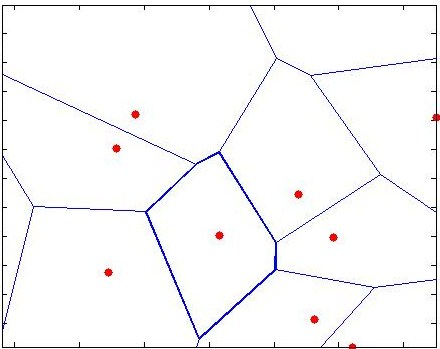
\includegraphics[width=2in]{vt.jpg}}
\end{columns} 
}

\frame{
\setbeamercovered{invisible}
\frametitle{CVT: facts and definitions}
\begin{itemize}
\item  Center of Mass: $C=\frac{\displaystyle \int_{v}\rho(y)y dy}{\displaystyle \int_{v}\rho(y) dy}$, where $\rho(y)$ is a density function
\item Define the Voronoi sets $V_{i},\,i=1,\dots,K$ corresponding to the given $\{z_{i}\}$ generators
\begin{itemize}
\item we can define the associated centroids $$z_{i}^{*},\,i=1,\dots,K$$
\end{itemize}
\item  In general, the centroids of the Voronoi sets don't coincide with the generators of the Voronoi sets, but if they do, i.e. $$z_{i}= z_{i}^{*},\, i=1,\dots,K$$  we call this kind of tessellation {\color{blue}Centroidal Voronoi Tessellation (CVT)}
\end{itemize}
}

\frame{
\frametitle{Examples of CVT}
\begin{center}
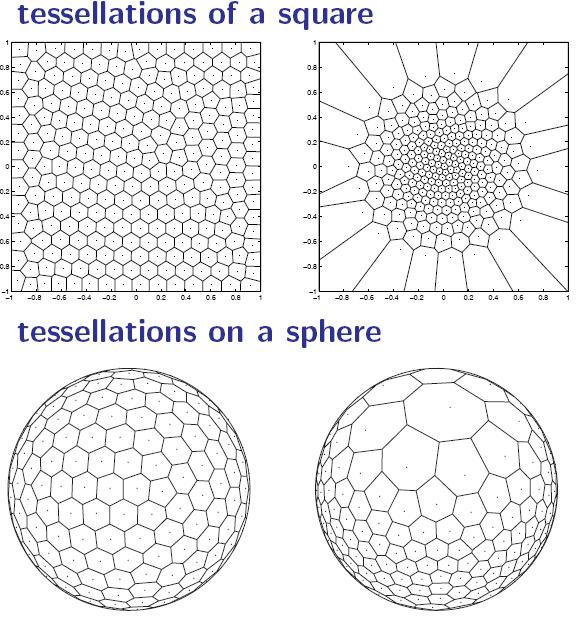
\includegraphics[width=2.8in]{CVTs.JPG}
\end{center}
}

\section{Applications}

\frame{
\frametitle{Range of applications}

\begin{itemize}
\item  Location optimization:\\
\begin{itemize}
\item optimal allocation of resources\\
\item mailboxes, bus stops, etc. in a city\\
\item distribution/manufacturing centers\\
\end{itemize}
\item Grain/cell growth
\item Crystal structure
\item Territorial behavior of animals
\item Data analysis:\\
\begin{itemize}
\item image compression, computer graphics, sound denoising etc\\
\item clustering gene expression data, stock market data
\end{itemize}
\item Engineering:\\
\begin{itemize}
\item vector quantization etc
\item Statistics (k-means):\\
\item classification, minimum variance clustering\\
\item data mining
\end{itemize}
\item Numerical methods\\
\begin{itemize}
\item Atmospheric and ocean modeling\\
\item Various other PDE solvers
\end{itemize} 
\end{itemize} 
}

\section{Lloyd method}
\subsection{Algorithm}
\frame{
\frametitle{Lloyd's algorithm to construct CVT's}
\begin{enumerate}
\item Start with the initial set of points $\{z_{i}\}_{i=1}^{K}$\\

\item Construct the Voronoi tessellation $\{V_{i}\}_{i=1}^{K}$ of $\Omega$ associated with the points $\{z_{i}\}_{i=1}^{K}$\\

\item Construct the centers of mass of the Voronoi regions $\{V_{i}\}_{i=1}^{K}$  found in Step 2; take centroids as the new set of points $\{z_{i}\}_{i=1}^{K}$\\

\item Go back to Step 2. Repeat until some convergence criterion is satisfied
\end{enumerate}
\begin{center}
\textcolor{red}{Note:Steps 2 and 3 can both be costly to effect}
\end{center}
}

\frame{
\frametitle{Illurstration of Lloyd's method}
\begin{columns}
\column{2.5in}
\centering
 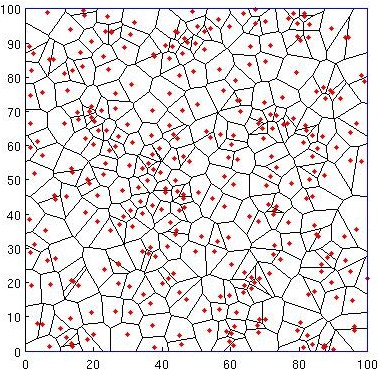
\includegraphics[width=2in]{first320exp.jpg}
\column{2.5in}
 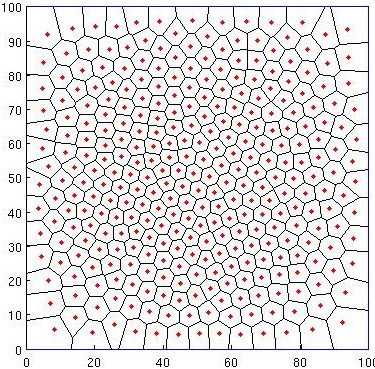
\includegraphics[width=2in]{final320exp.jpg}
\end{columns}
}

\frame{
\frametitle{Convergence result of Lloyd's method}
\begin{itemize}
\item Lloyd method has \textcolor{red}{linear convergence rate: $\|error_{k+1}\| \approx r \|error_{k}\|$}\\

\item For strongly log-concave densities, $$r \approx 1-\frac{C}{K^2}
$$
\item very slow if $K$ large.
\end{itemize}

\begin{center}
{\bf Is speedup possible?}
\end{center}			       
}

\section{Appliction of MG/OPT on CVT}
\subsection{Multilevel approach to construct CVT}
\frame{
\frametitle{Multilevel approach to construct CVT}
\begin{itemize}
\item Given generators $\bzin$  and the corresponding tessellation $\vin$, define the {\em energy functional}
$$ \label{ener}
{\cg}\Bigl(\bzin\Bigr)
=
\sum_{i=1}^k  \int_{\vi} \rho(\by)|\by - \bzi|^2 \,d\by.
$$\\

\item The minimizer of $\cg$ necessarily forms a CVT \\

\item We treat CVT as a minimization problem and apply a multilevel optimization framework called MG/OPT to this functional
\item The multilevel framework uses coarse approximations to $\cg$ to accelerate a traditional optimization algorithm (OPT)
\end{itemize}
}

\subsection{Introduction of MG/OPT}
\frame{
\frametitle{Multilevel Algorithm: MG/OPT [S.G.Nash 2000]}
\begin{itemize}
\item Given:
\begin{itemize}
\item Traditional optimization algorithm OPT
\item Downdate and update operators
\item Integers $k_{1}$ and $k_{2}$ satisfying $k_{1}+k_{2}>0$
\end{itemize}

\item One iteration of MG/OPT:
\begin{itemize}
\item Pre-smoothing: Apply $k_{1}$ iterations of OPT to the fine energy function
\item Recursion: 
\begin{itemize}
\item Downdate the generators
\item Apply MG/OPT to a shifted version of the coarse energy function
\item Use result to update the generators on the fine level
\end{itemize}
\item Post-smoothing: Apply $k_{2}$ iterations of OPT to the fine energy function
\end{itemize}
\end{itemize}
}






\subsection{Convergence result of MG/OPT on 1-D CVT}
\frame{
\frametitle{Convergence result of MG/OPT on 1-D CVT}
\begin{center}
Red: Opt;   Blue: MG/OPT; $\rho(x)=1$
\end{center}
\begin{center}
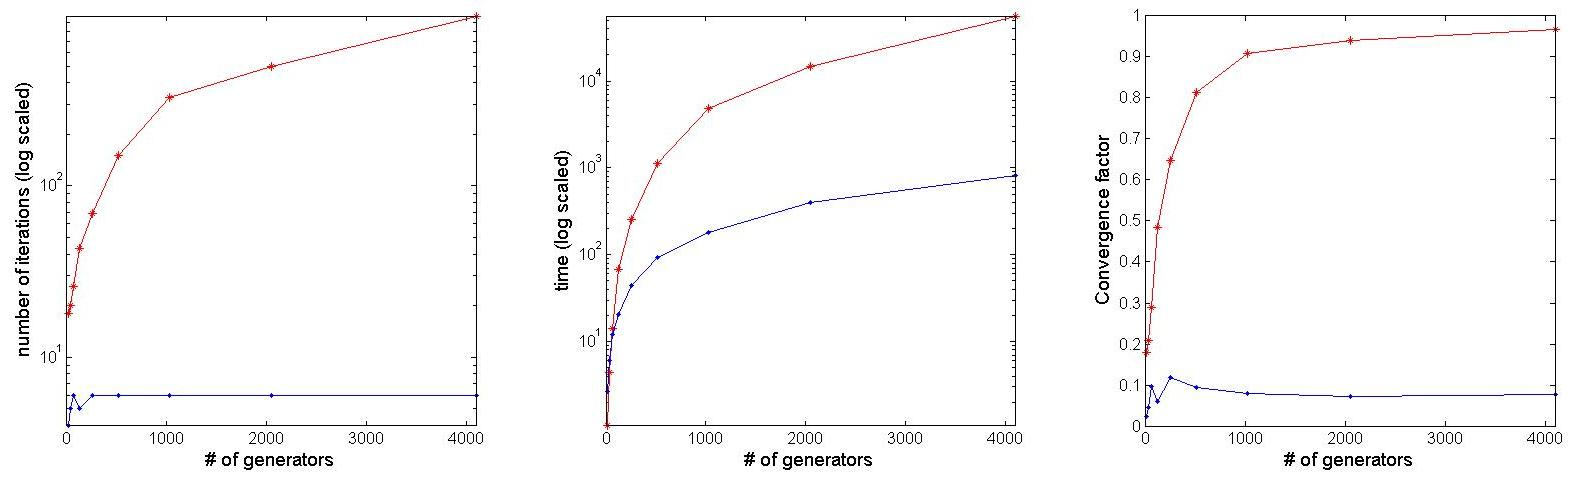
\includegraphics[width=4.8in]{graph_unioptmg.jpg}
\end{center}
\onslide<2->{\footnotesize{ For more information, please read our paper: ''Truncated Newton-based multigrid algorithm for centroidal Voronoi calculation", Z. Di, M. Emelianenko and
S. Nash}}
}

\section{Summary}
\frame{
\frametitle{Discussion}
\textcolor{blue}{Results and challenges:}
\begin{itemize}

\item CVT is in the heart of many applications and the number is growing:\\
computer science, physics, social sciences, biology, engineering ...

\item The main advantage of MG/OPT is its superior convergence speed when compared to other existing approaches.

\item The simplicity of its design and the results of preliminary tests suggest that the method is generalizable to higher dimensions, which is the subject of current investigations

\item Future work also includes application of this technique to various scientific and engineering applications, including image analysis and grid generation.
\end{itemize}
\onslide<2->
{\begin{center}
\textcolor{red}{THANKS!}
\end{center}
}
}
\end{document}

